\chapter{From Climate Change Uncertainty to Climate Change Ambiguity}


\section{Population Modelling}


\begin{figure}
\centering
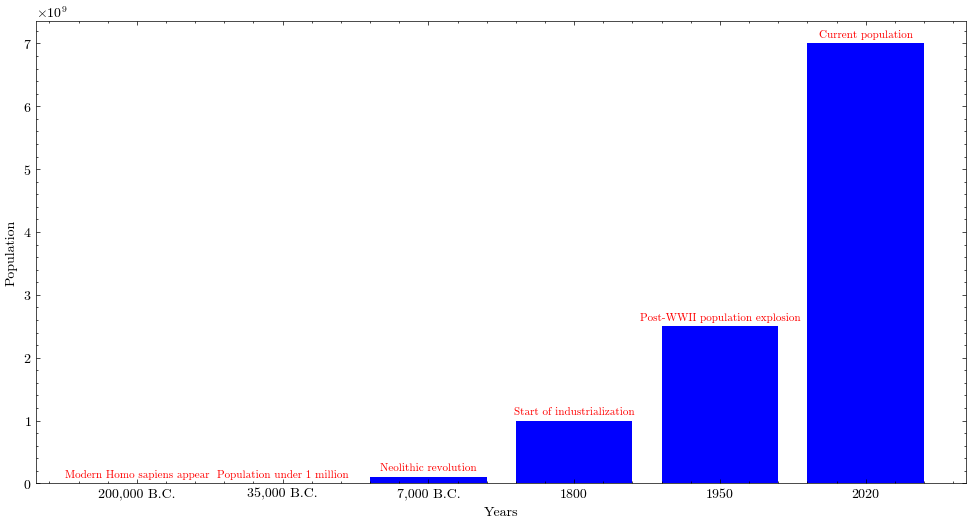
\includegraphics[width=1\textwidth]{../images/population/history_population.png}
\caption{History of Human Population Growth}
\label{fig:population}
\end{figure}

The scientific discipline of demography 
produces detailed population projections based 
assumptions about the future trend in fertilty,
mortality and migration.

\subsection{Key Dimensions of Population Modelling}

Two important reasons to go beyond population size. 
Human population is not homogenous. And this 
heterogeneity is important for future growth 
of the population. Population growth is a 
direct function of the age and sex 
structure of the population.

\subsection{Educational Fertility Differential}

Total Fertility Rate (TFR)

Education-Specific TFR (ESTFR)

Age-Specific Fertility Rate (ASFR)

Education-Specific Age-Specific Fertility Rate (ESASFR)

Parametric model: 
specify ASFR relative to a reference distribution. 
The reference or standard ASFR can be 
described by a Gompertz function. This 
is an s-shaped function similar to a 
logistic function, but it is asymmetric, 
with faster growth at the beginning and
slower growth at the end.

Age refer to the transformed age. The Gompit is 
defined as:

\begin{equation}
    Y(x) = -log(-log(x))
\end{equation}

With $F(x)$ the cumulative distribution of the ASFR 
at age $x$:

\begin{equation}
F(x) = \int_{0}^{x} \frac{ASFR(y)}{TFR}dy
\end{equation}

\subsection{Educational Mortality Differential}


\subsection{Education Scenarios}